\documentclass[12pt]{article}
\usepackage[dvips]{epsfig}
\usepackage{color}
\usepackage{url}
\usepackage[colorlinks=true]{hyperref}

\begin{document}

\section*{GENESIS: Documentation}

{\bf Related Documentation:}
% start: userdocs-tag-replace-items related-do-nothing
% end: userdocs-tag-replace-items related-do-nothing

\section*{The {\it Developer} Package}

Maintaining many software projects quickly becomes a lot of work.  It
also makes it difficult for new people to step into software
development, for example, because dependency tracking between software
components must be done manually.  The {\it Developer} package
automates the management of multiple software projects.  It automates
updates to local source code, synchronization between distributed
repositories, compilation, testing and installation, packaging and
releases, serving monotone repositories and other things.  Besides
monotone it also has experimental support for integration with
mercurial.

The {\it Developer} package provides developer utilities that comply with GENESIS development standards. The most important one is the {\it
  neurospaces\_build} script used for automated software installation and maintenance on a configurable set of software packages.  Because
this script has many options, most common operations are provided using frontends.  Other scripts are related to version identification of the software, source code documentation comments, testing, and release management. The following sections include simple and detailed examples. 

\subsection*{Downloading the  {\it Developer} Package}
The {\it Developer} Package can be downloaded from the \href{http://sourceforge.net/projects/neurospaces/files/}{\bf Neurospaces Project} website.

\subsection*{Simple Examples}
Simple examples can be used by developers who do not want to know about the intricate details of the {\it Developer} tools.  Most developers fall into this category. Software developers and laboratories who have added their own private software components should be OK using the simple examples and can skip reading the detailed examples.

\subsection*{Detailed Examples}
The detailed examples provide:
\begin{itemize}
   \item[]Steps to build a release for the example {\tt <your-software>} package.
   \item[]Examples of the release procedure.
\end{itemize}

\subsection*{Utilities}
Some utilities currently depend on \href{http://monotone.ca}{monotone} for source code version control due to their configuration. It is possible to work with other version control systems.

\subsubsection*{Main script}

\begin{itemize}
   \item {\it neurospaces\_build}:\,\,\,Performs various back-end operations on a set of software packages. It is configurable in its packages and operations. The command:
      \begin{verbatim}
   neurospaces_build --help
      \end{verbatim}
describes how the script works and lists default actions and build options. The flags at the end of the output should be inspected.

   \item {\bf In brief:} {\it neurospaces\_build} operates in one of two modes determined by where the script finds the source code (``{\tt neurospaces\_build --help}'' gives more details). As indicated in the following figure, {\it neurospaces\_build} creates an extensible associative array (hash table) that can be visualized as a matrix of packages (rows) and build operations (columns). The script traverses the matrix by row, i.e. packages first, and performs successive build operations for a given package. The figure below  lists the default build options. Options to {\it neurospaces\_build} select or deselect cells in the matrix according to the configuration specified by any options to the {\it neurospaces\_build} command. {\bf Note:} Addition of a new component to GENESIS is the equivalent of adding a new column to the {\it neurospaces\_build} associative matrix.
   
\begin{figure}[h]
   \centering
   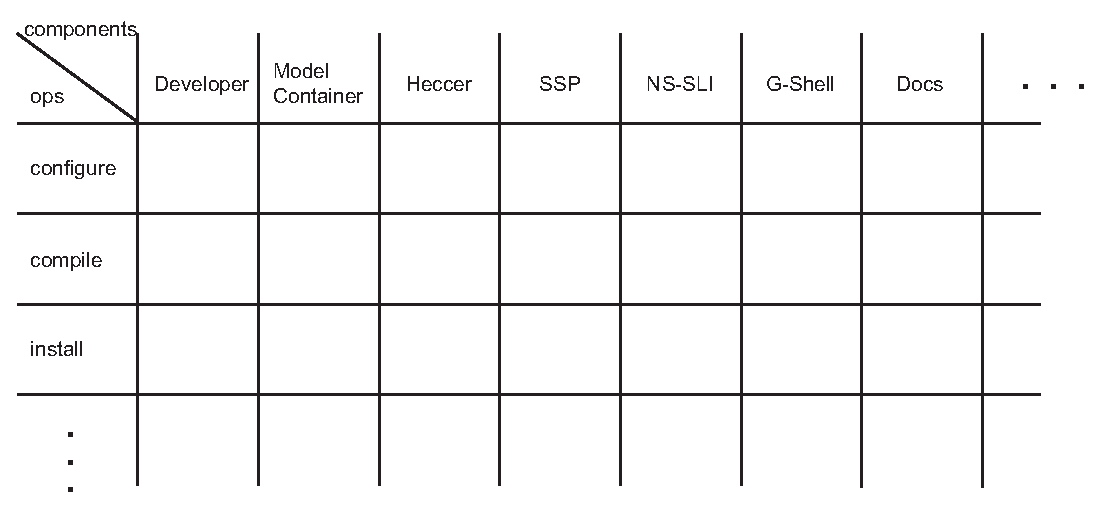
\includegraphics[scale=0.7]{figures/build-matrix.eps}
%   \caption{{\bf A Dummy Figure:} Example of Latex code to incorporate
%      a figure into documentation.}
%   \label{fig:df-1}
\end{figure}
   
   \item {\bf Installation Order of Components:} This is the left -$>$ right component order in the {\it neurospaces\_build} associative array:
   \begin{enumerate}
      \item {\it Developer} {\bf Component:} Described in this documentation.
      \item \href{../model-container/model-container.tex}{\bf Model\,Container:} Provides a highly optimized solver-independent internal storage format for models.
      \item \href{../exchange/exchange.tex}{\bf Exchange:} Provides exchange in common descriptive standards such as NeuroML and NineML.
      \item \href{../heccer/heccer.tex}{\bf Heccer:} The current standard numerical solver.
      \item \href{../ssp/ssp.tex}{\bf SSP:} The simple Scheduler in Perl is currently the standard scheduler for GENESIS.
      \item \href{../ns-sli/ns-sli.tex}{\bf NS-SLI:} The GENESIS 2 Backward Compatibility Module. Required to run GENESIS 2 scripts.
      \item \href{../gshell/gshell.tex}{\bf G-Shell:} Runs interactive GENESIS sessions.
      \item \href{../documentation-overview/documentation-overview.tex}{\bf GENESIS Documentation System:} A modular documentation system designed to maintain geographically distributed software systems.
   \end{enumerate}
   \item {\bf Note:} When installing GENESIS manually, it is recommended to follow the installation order given above. 
\end{itemize}

%Also look at \href{../release-procedure/release-procedure.tex}{ReleaseProcedure}.

\subsubsection*{Front-end {\it Developer} Scripts}

The following utilities take optional arguments of ``{\tt --regex}'' to select the packages they operate on, and ``{\tt --verbose}'' to run the command in a more verbose mode. They follow the order of the \href{../workflow-developer/workflow-developer.tex}{Developer\,Workflow}. The information they return are determined by the configuration of the {\it Developer} package.

{\bf Note:} These {\it Developer} package commands are run from a command line prompt, i.e. outside the GENESIS environment.

\begin{enumerate}
   \item {\bf Write/Update Code:}
   \begin{itemize}
      \item {\it neurospaces\_create\_directories}\,\,\,Create the correct directory layout required for GENESIS development.
      \item {\it neurospaces\_download}\,\,\,Download GENESIS components from a central archive.
      \item {\it neurospaces\_init}\,\,\,Create source code repositories.
      \item {\it neurospaces\_pull}\,\,\,Download the source code or patches from a remote repository. This places the newest version of the source 
      code in your local repository.
      \item {\it neurospaces\_push}\,\,\,Upload source code or patches to a remote repository.
      \item {\it neurospaces\_serve}\,\,\,Starts serving the source code repositories such that other people can {\it pull} and {\it sync} to your machine (note that this locks all your local databases).
      \item {\it neurospaces\_status}\,\,\,Check for local source code modification (no network required).
      \item {\it neurospaces\_sync}\,\,\,Synchronize local source code modification with a repository.
      \item {\it neurospaces\_update}\,\,\,Makes the local source code up to date using the repositories locally stored on your PC (so this is an entirely local operation). If necessary, this command also automatically merges parallel development branches.
      \item {\it neurospaces\_upgrade}\,\,\,Pulls code from the GENESIS repositories, calls {\it neurospaces\_update} and {\it neurospaces\_install}
      \item {\it neurospaces\_tools\_propagate}\,\,\,Propagates updates to source code of shared tools from source to target packages.
   \end{itemize}
  
   \item{\bf Document Code API:}
   \begin{itemize}
      \item {\it mcad2doxy}\,\,\,Convert obsolete multicad documentation to {\it doxygen} format, this has been used to convert the {\bf Heccer} 
      developer documentation to {\it doxygen} format. Other packages will follow.
      \item {\it neurospaces\_docs}\,\,\,Builds documentation on your local machine.
      \item {\it neurospaces\_website\_prepare}\,\,\,Prepare a version of the website on your local PC, and optionally upload it. 
   \end{itemize}
  
   \item{\bf Build/Check:}
   \begin{itemize}
      \item {\it neurospaces\_configure}\,\,\,(Re)configures the simulator software (requires packages to be installed already).
      \item {\it neurospaces\_install}\,\,\,Install new simulator executable binaries and scripts.
      \item {\it neurospaces\_uninstall}\,\,\,Uninstalls the simulator software (including the installer scripts, to reinstall you must go to the {\it Developer} source code directory and run ``{\tt make \&\& sudo make install}'').
      \item {\it neurospaces\_clean}\,\,\,Clean local source code directories. 
   \end{itemize}
  
   The {\it neurospaces\_upgrade} command makes the local source code
   up to date with the source code served by the remote servers.  It
   thereby combines steps 1 and 3 explained above.  This command is
   similar in operation to the invocation of the commands {\it
     neurospaces\_uninstall}, {\it neurospaces\_pull}, {\it
     neurospaces\_clean}, {\it neurospaces\_update}, {\it
     neurospaces\_install}

   \item {\bf Regression Testing:}
   \begin{itemize}
      \item {\it nstest\_query}\,\,\,Queries test specifications of a package.
      \item {\it neurospaces\_harness}\,\,\,Run the test specifications found in the current directory, see also \href{../neurospaces-tester/neurospaces-tester.tex}{the Neurospaces tester}.
      \item {\it neurospaces\_check}\,\,\,Check for correctness of the installed software.
      \item{\bf Simple Example:} Enable the {\it distcheck} target of the {\it make} files, in addition to the default actions:
      \begin{verbatim}
   $ neurospaces_build --distcheck --help
      \end{verbatim}
   \end{itemize}
 
   \item {\bf Internal/Public Release:}
   \begin{itemize}
      \item {\it nspkg-deb}\,\,\,Automated debian package builder.
      \item {\it neurospaces\_packages}\,\,\,Show which packages are enabled on your local machine.
      \item{\bf Simple Example:} This command invokes 
      \begin{verbatim}
   $ neurospaces_build --help-packages
      \end{verbatim}
      \item {\it neurospaces\_dist}\,\,\,Build a release given a milestone label and version number. This script also inserts the milestone label and version number into the Tag database which is a YAML file and can be found at: {\it /etc/neurospaces/tag\_database}. The following two utilities query this database:
      \begin{itemize}
         \item {\it td-labels}\,\,\,Shows all release labels (major and version numbers).
         \item {\it td-majors}\,\,\,Shows all major release labels.
      \end{itemize}

For updating of version keywords the following are invoked automatically by the {\it neurospaces\_build} script:
   \begin{itemize}
       \item {\it release\_extract}\,\,\,Extract release information from a monotone repository. When a Tag is set, that will be the result, otherwise the SHA of the current base revision will be the result.
      \item {\it release\_expand}\,\,\,Do keyword expansion, see the {\it manpage} in the source for more details.
   \end{itemize}
      \item{\bf Simple Example:} What shell commands will be run after options have been given, without really running the commands.
\begin{verbatim}
   $ neurospaces_build --verbose --distcheck --dry-run --developer
\end{verbatim}
      \item{\bf Simple Example:} How are operations mapped to packages.
\begin{verbatim}
   $ neurospaces_build --help-all
\end{verbatim}
      \item{\bf Detailed Example:} Steps in building a release for the example {\tt <your-software>} package.
      \begin{itemize}
         \item {\bf Tag the code:} The GENESIS convention for creating these tags, which must be unique, is to concatenate an identifier from the name of the lab of origin, the purpose and/or type of software (e.g. build, passive, active, python, userdocs, des, network, i64, purkinje, integration, pools, etc), with an appended numerical identifier. Here, for example we use the generic tag ``{\tt <mylab-mysoftware-vnum>}''.
\begin{verbatim}
   $ neurospaces_build --tag <mylab-mysoftware-vnum> --verbose --verbose --verbose --no-compile --no-configure --no-install --regex <my-software> --developer
\end{verbatim}

         \item {\bf Build the release for the tagged code:}
\begin{verbatim}
   $ neurospaces_build --dist --verbose --verbose --verbose --no-compile --no-configure --no-install --regex <my-software> --developer
\end{verbatim}

         \item {\bf Or with one command line:}
\begin{verbatim}
   $ neurospaces_build --tag <mylab-mysoftware-vnum> --dist --verbose --verbose --verbose --no-compile --no-configure --no-install --regex <my-software> --developer
\end{verbatim}

         \item {\bf Upload the tarballs:}
\begin{verbatim}
   $ neurospaces_build --src-tag <mylab-mysoftware-vnum> --upload-server ftp://upload.sourceforge.net/incoming --verbose --verbose --verbose --no-compile --no-configure --no-install --regex <my-software> --developer
\end{verbatim}
Do not forget to edit release notes, tag the files as ``Any'', ``Source.gz'', etc. Due to the crappy Sourceforge interfaces, this has to be done manually (anyone have any ideas?).
      
   \end{itemize}
\end{itemize}
  
   \item {\bf Integrate Software Components:}
   \begin{itemize}
      \item {\it neurospaces\_versions}\,\,\,Shows which versions of the GENESIS packages are installed.
      \item \href{../neurospaces-cron/neurospaces-cron.tex}{\it neurospaces\_cron}\,\,\,A {\it cron} job based tester script. 
      \item {\bf Simple Example:} What operations on known packages exist.
      \begin{verbatim}
   $ neurospaces_build --help-operations
      \end{verbatim}
   \end{itemize}

\end{enumerate}

\subsection*{Detailed Examples of the Release Procedure}

After putting a Tag on the code, you first must check if the package can be built from the tarball. The autotools {\it distcheck} target does this (see below). An additional check is to build the tarball, put it somewhere on your filesystem, and then build the {\it check} target from the tarball. For example, first build the tarball and put it somewhere on your filesystem (e.g. {\it /tmp/uploads}):
\begin{verbatim}
   neurospaces_build --developer --verbose --upload-server --no-install --regex studio
\end{verbatim}
Then build the {\it check} target from the tarball:
\begin{verbatim}
   neurospaces_build --verbose --check --regex studio --src-tag python-5  --src-dir /tmp/uploads --verbose --verbose --unpack --no-install
\end{verbatim}
In a one line summary you need to insert a {\tt --tag}, and {\tt --distcheck} the current code, then make them available on \href{http://sourceforge.net/projects/neurospaces/}{Sourceforge}. In one line of code:
\begin{verbatim}
   neurospaces_build --developer --distcheck --verbose --tag network-5 --src-tag network-5 --upload-server https://frs.sourceforge.net/uploads --verbose
\end{verbatim}
If you don't want to do the upload, for a single package:
\begin{verbatim}
   neurospaces_build --tag network-5 --distcheck --regex 'model-container' --developer --verbose
\end{verbatim}
If that works, you then want to do the upload:
\begin{verbatim}
   neurospaces_build --src-tag network-5 --upload-server https://frs.sourceforge.net/uploads --regex 'model-container' --developer --verbose
\end{verbatim}
The {\tt --verbose} option is there to let you know what is going on during this lengthy procedure.

The same procedure is used to build a release of either individual or all packages. An official public release is made available for download on \href{http://sourceforge.net/projects/neurospaces/}{Sourceforge}. Intermediate releases are for internal use only.

Because official releases are built using automake's {\it distcheck} target, they must pass the tests of the package (on the machine used for the build). So they are considered to be alpha releases (ie. internally well tested).

The release procedure normally checks for package correctness using the automake {\it distcheck} target, meaning that both install and uninstall targets work and are each other's complement. Official releases must always succeed on this target. Intermediate releases can fail.


\subsubsection*{Other Examples}

\begin{itemize}
\item {\bf Uninstall 4 packages on your developer machine:}
\begin{verbatim}
   $ neurospaces_build --verbose --verbose --verbose --no-compile --no-configure --uninstall --regex '(my-software|heccer|ssp|studio)' --developer
\end{verbatim}

\item {\bf Build checked releases for four packages:}
\begin{verbatim}
   $ neurospaces_build --verbose --verbose --verbose --no-compile --no-configure --no-install --distcheck --regex '(my-software|heccer|ssp|studio)' --developer
\end{verbatim}

\item {\bf After a modification of the developer package, reinstall it:}
\begin{verbatim}
   $ neurospaces_build --enable developer --regex developer --developer --verbose --verbose --verbose
\end{verbatim}

\item {\bf Releasing the developer package on Sourceforge:}
\begin{verbatim}
   $ neurospaces_build --tag build-25 --dist --src-tag build-25 --upload-server ftp://upload.sourceforge.net/incoming --enable developer --regex '(developer)' --developer --verbose
\end{verbatim}
\end{itemize}

\end{document}
